\chapter{REVISÃO DE LITERATURA}
\label{chp:capitulo2}

Em um campo com uma quantia tão rarefeita de artigos, publicações e materiais em larga parte espalhadas por blogs na internet, foi necessário realizar uma revisão de literatura para que as ferramentas de ponta, estratégias ainda sendo testadas e vulnerabilidades principais no mercado fossem corretamente identificadas. Isso se torna especialmente verdadeiro pela mudança no cenário de segurança dos anos 2000 para os anos 2010-2022, aonde boa parte de ameaças antigas podem ser de pouca relevância.

Aqui serão amostrados alguns dos principais achados, as estratégias para organizar os mesmos e resumido o estado da arte no presente momento.

\section{Levantamento de Artigos - Ferramentas empregadas}
\subsection{Parsifal}
Parsifal é uma ferramenta originalmente designada para realizar Revisões Sistemáticas de Literatura, que embora sejam de escopo maior que a revisão rápida que foi realizada neste trabalho, ainda contou com uma série de funcionalidades que permitisse catalogar, processar e essencialmente medir o progresso das pesquisas realizadas no assunto.

\begin{figure}[ht]
    \centering
    \caption{Dashboard Parsifal}
    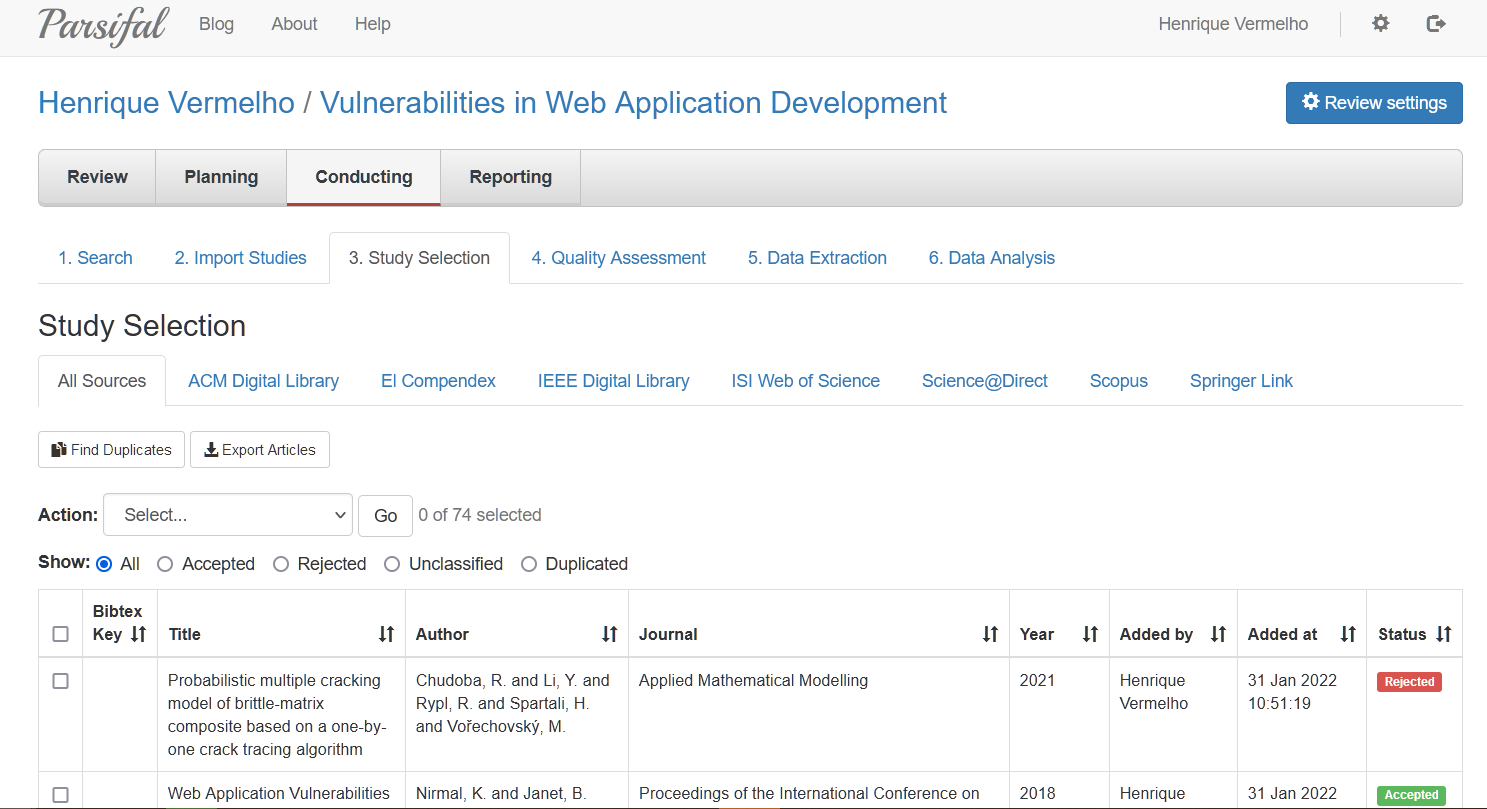
\includegraphics[width=16cm]{figuras/parsifal.png} 
    \legend{Fonte: \href{https://parsif.al}{parsif.al} (2022, p. TO-DO)}
    \label{fig:internet} 
\end{figure}

Na figura acima pode-se verificar no topo quatro abas principais - \textbf{Review, Planning, Conducting, }e \textbf{Reporting}.


\subsection{Scopus + CAFe},
scopus, levantamento de artigos e estado da arte

\section{nscanner}

\section{WAF-A-MoLE}

\subsection{Linear SVM}

\subsection{Seção Terciária}

Alíneas e subalíneas.
\bigskip

\begin{alineas}
\item linha 1:
\begin{alineas}
\item subalinea 1;
\item subalinea 2;
\end{alineas}
\item linha 2:
\begin{subalineas}
\item subalinea 1;
\item subalinea 2;
\end{subalineas}
\item linha 3:
\begin{incisos}
\item subalinea 1;
\item subalinea 2;
\end{incisos}
\item linha 4.
\end{alineas}

